\documentclass[hyphens,aspectratio=169]{beamer}
\usepackage{graphicx}
\usepackage{amssymb}
\usepackage{amsmath}
\usepackage{mathtools}
\usepackage{textcomp}
\usepackage{moresize}
\usepackage{framed}
\usepackage{minted}
\usepackage{relsize}
\usepackage{tikz}
\usetikzlibrary{positioning}

\usetheme{Berlin}
\usecolortheme[RGB={0,95,47}]{structure}
\beamertemplatenavigationsymbolsempty

\makeatletter
\AtBeginEnvironment{minted}{\dontdofcolorbox}
\def\dontdofcolorbox{\renewcommand\fcolorbox[4][]{##4}}
\makeatother

\begin{document}

\begin{frame}[fragile]{The Stack}
    \begin{itemize}
        \pause \item The stack is a RW region of memory that is present at process initialization time.
        \pause \item At initialization time, \texttt{rsp} contains an address within the stack.
        \pause \item The stack is often used as a stack (as in, the data structure).
    \end{itemize}
\end{frame}

\begin{frame}[fragile]{The Stack}
    Things that usually go on the stack:
    \begin{itemize}
        \pause \item Local variables
        \pause \item Function return addresses
    \end{itemize}
\end{frame}

\begin{frame}[fragile]{Why do function return addresses go on the stack?}
    \begin{columns}
        \begin{column}{0.5\textwidth}
            Consider the following C program:
                \inputminted[fontsize=\tiny]{c}{call.c}
        \end{column}
        \begin{column}{0.5\textwidth}
            \pause This is its \textit{call graph}:
            \vspace{1cm}

            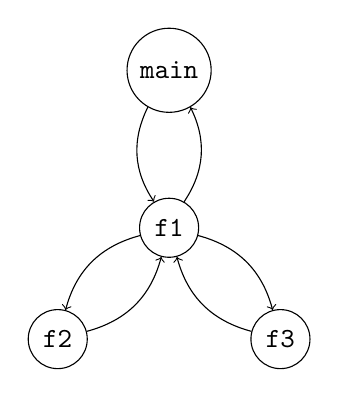
\begin{tikzpicture}[node distance=2cm]
                \node[circle, draw] (main) {\texttt{main}};
                \node[circle, draw, below of=main] (f1) {\texttt{f1}};
                \node[circle, draw, below left of=f1] (f2) {\texttt{f2}};
                \node[circle, draw, below right of=f1] (f3) {\texttt{f3}};

                \path[every node/.style={font=\sffamily\small}]
                    (main) edge[->, bend right] (f1)
                    (f1) edge[->, bend right] (f2)
                    (f2) edge[->, bend right] (f1)
                    (f1) edge[->, bend left] (f3)
                    (f3) edge[->, bend left] (f1)
                    (f1) edge[->, bend right] (main)
                    ;
            \end{tikzpicture}
        \end{column}
    \end{columns}
\end{frame}

\begin{frame}[fragile]{Why do function return addresses go on the stack?}
    \begin{columns}
        \begin{column}{0.5\textwidth}
            Consider the following C program:
                \inputminted[fontsize=\tiny]{c}{call.c}
        \end{column}
        \begin{column}{0.5\textwidth}
            This is its \textit{call graph}:
            \vspace{1cm}

            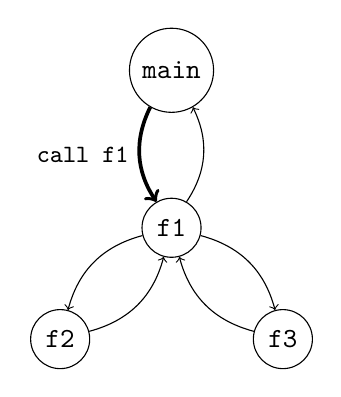
\begin{tikzpicture}[node distance=2cm]
                \node[circle, draw] (main) {\texttt{main}};
                \node[circle, draw, below of=main] (f1) {\texttt{f1}};
                \node[circle, draw, below left of=f1] (f2) {\texttt{f2}};
                \node[circle, draw, below right of=f1] (f3) {\texttt{f3}};

                \path[every node/.style={font=\sffamily\small}]
                    (main) edge[->, bend right, line width=1.34pt] node[left] {\texttt{call f1}} (f1)
                    (f1) edge[->, bend right] (f2)
                    (f2) edge[->, bend right] (f1)
                    (f1) edge[->, bend left] (f3)
                    (f3) edge[->, bend left] (f1)
                    (f1) edge[->, bend right] (main)
                    ;
            \end{tikzpicture}
        \end{column}
    \end{columns}
\end{frame}

\begin{frame}[fragile]{Why do function return addresses go on the stack?}
    \begin{columns}
        \begin{column}{0.5\textwidth}
            Consider the following C program:
                \inputminted[fontsize=\tiny]{c}{call.c}
        \end{column}
        \begin{column}{0.5\textwidth}
            This is its \textit{call graph}:
            \vspace{1cm}

            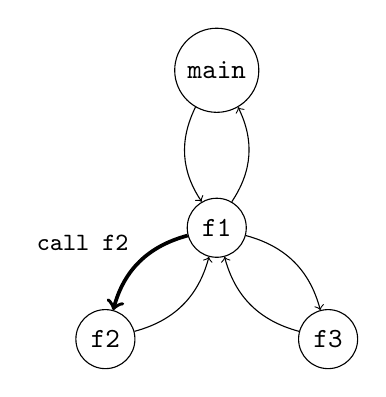
\begin{tikzpicture}[node distance=2cm]
                \node[circle, draw] (main) {\texttt{main}};
                \node[circle, draw, below of=main] (f1) {\texttt{f1}};
                \node[circle, draw, below left of=f1] (f2) {\texttt{f2}};
                \node[circle, draw, below right of=f1] (f3) {\texttt{f3}};

                \path[every node/.style={font=\sffamily\small}]
                    (main) edge[->, bend right] (f1)
                    (f1) edge[->, bend right, line width=1.34pt] node[above left] {\texttt{call f2}} (f2)
                    (f2) edge[->, bend right] (f1)
                    (f1) edge[->, bend left] (f3)
                    (f3) edge[->, bend left] (f1)
                    (f1) edge[->, bend right] (main)
                    ;
            \end{tikzpicture}
        \end{column}
    \end{columns}
\end{frame}

\begin{frame}[fragile]{Why do function return addresses go on the stack?}
    \begin{columns}
        \begin{column}{0.5\textwidth}
            Consider the following C program:
                \inputminted[fontsize=\tiny]{c}{call.c}
        \end{column}
        \begin{column}{0.5\textwidth}
            This is its \textit{call graph}:
            \vspace{1cm}

            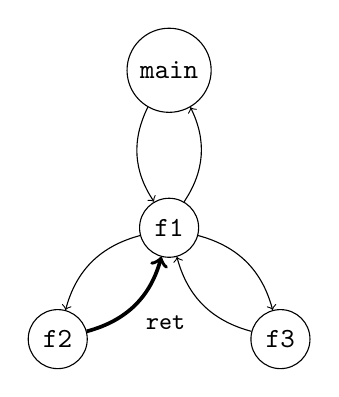
\begin{tikzpicture}[node distance=2cm]
                \node[circle, draw] (main) {\texttt{main}};
                \node[circle, draw, below of=main] (f1) {\texttt{f1}};
                \node[circle, draw, below left of=f1] (f2) {\texttt{f2}};
                \node[circle, draw, below right of=f1] (f3) {\texttt{f3}};

                \path[every node/.style={font=\sffamily\small}]
                    (main) edge[->, bend right] (f1)
                    (f1) edge[->, bend right] (f2)
                    (f2) edge[->, bend right, line width=1.34pt] node[below right] {\texttt{ret}} (f1)
                    (f1) edge[->, bend left] (f3)
                    (f3) edge[->, bend left] (f1)
                    (f1) edge[->, bend right] (main)
                    ;
            \end{tikzpicture}
        \end{column}
    \end{columns}
\end{frame}

\begin{frame}[fragile]{Why do function return addresses go on the stack?}
    \begin{columns}
        \begin{column}{0.5\textwidth}
            Consider the following C program:
                \inputminted[fontsize=\tiny]{c}{call.c}
        \end{column}
        \begin{column}{0.5\textwidth}
            This is its \textit{call graph}:
            \vspace{1cm}

            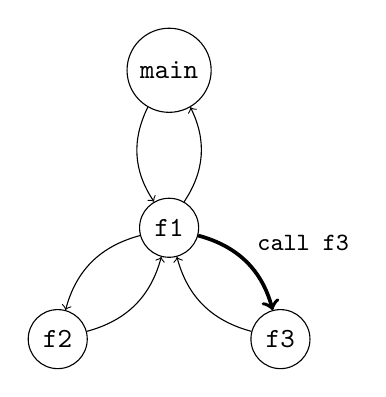
\begin{tikzpicture}[node distance=2cm]
                \node[circle, draw] (main) {\texttt{main}};
                \node[circle, draw, below of=main] (f1) {\texttt{f1}};
                \node[circle, draw, below left of=f1] (f2) {\texttt{f2}};
                \node[circle, draw, below right of=f1] (f3) {\texttt{f3}};

                \path[every node/.style={font=\sffamily\small}]
                    (main) edge[->, bend right] (f1)
                    (f1) edge[->, bend right] (f2)
                    (f2) edge[->, bend right] (f1)
                    (f1) edge[->, bend left, line width=1.34pt] node[above right] {\texttt{call f3}} (f3)
                    (f3) edge[->, bend left] (f1)
                    (f1) edge[->, bend right] (main)
                    ;
            \end{tikzpicture}
        \end{column}
    \end{columns}
\end{frame}

\begin{frame}[fragile]{Why do function return addresses go on the stack?}
    \begin{columns}
        \begin{column}{0.5\textwidth}
            Consider the following C program:
                \inputminted[fontsize=\tiny]{c}{call.c}
        \end{column}
        \begin{column}{0.5\textwidth}
            This is its \textit{call graph}:
            \vspace{1cm}

            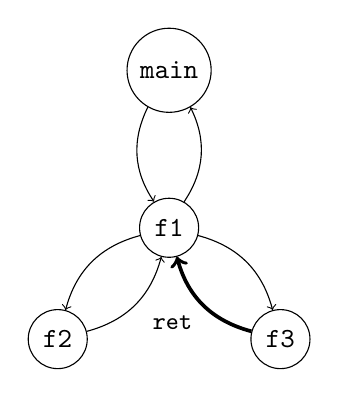
\begin{tikzpicture}[node distance=2cm]
                \node[circle, draw] (main) {\texttt{main}};
                \node[circle, draw, below of=main] (f1) {\texttt{f1}};
                \node[circle, draw, below left of=f1] (f2) {\texttt{f2}};
                \node[circle, draw, below right of=f1] (f3) {\texttt{f3}};

                \path[every node/.style={font=\sffamily\small}]
                    (main) edge[->, bend right] (f1)
                    (f1) edge[->, bend right] (f2)
                    (f2) edge[->, bend right] (f1)
                    (f1) edge[->, bend left] (f3)
                    (f3) edge[->, bend left, line width=1.34pt] node[below left] {\texttt{ret}} (f1)
                    (f1) edge[->, bend right] (main)
                    ;
            \end{tikzpicture}
        \end{column}
    \end{columns}
\end{frame}

\begin{frame}[fragile]{Why do function return addresses go on the stack?}
    \begin{columns}
        \begin{column}{0.5\textwidth}
            Consider the following C program:
                \inputminted[fontsize=\tiny]{c}{call.c}
        \end{column}
        \begin{column}{0.5\textwidth}
            This is its \textit{call graph}:
            \vspace{1cm}

            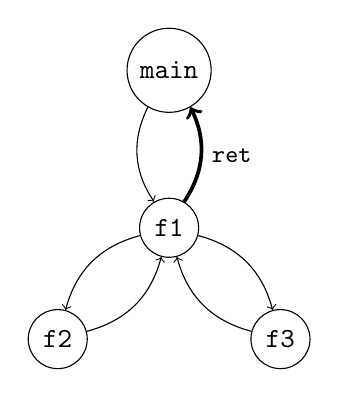
\begin{tikzpicture}[node distance=2cm]
                \node[circle, draw] (main) {\texttt{main}};
                \node[circle, draw, below of=main] (f1) {\texttt{f1}};
                \node[circle, draw, below left of=f1] (f2) {\texttt{f2}};
                \node[circle, draw, below right of=f1] (f3) {\texttt{f3}};

                \path[every node/.style={font=\sffamily\small}]
                    (main) edge[->, bend right] (f1)
                    (f1) edge[->, bend right] (f2)
                    (f2) edge[->, bend right] (f1)
                    (f1) edge[->, bend left] (f3)
                    (f3) edge[->, bend left] (f1)
                    (f1) edge[->, bend right, line width=1.34pt] node[right] {\texttt{ret}} (main)
                    ;
            \end{tikzpicture}
        \end{column}
    \end{columns}
\end{frame}

\begin{frame}[fragile]{Is this familiar?}
    \pause \begin{center}It's DFS!\end{center}
\end{frame}

\begin{frame}[fragile]{Why do local variables go on the stack?}
    \begin{itemize}
        \pause \item Q: Why use the stack for locals? Why not instead dedicate a fixed memory address for each local variable in each function?
        \pause \item A: Recursion! If a function calls itself, we need to store multiple copies of each local variable in the function.
        \pause \item For this reason, locals are also stored on the stack.
    \end{itemize}
\end{frame}

\begin{frame}[fragile]{Stack-Related Instructions}
    \begin{itemize}
        \pause \item \texttt{push some\_operand}. Equivalent to
            \begin{itemize}
                \pause \item \texttt{sub rsp, 8}, followed by
                \pause \item \texttt{mov QWORD PTR [rsp], some\_operand}.
            \end{itemize}
        \pause \item \texttt{pop some\_operand}. Equivalent to
            \begin{itemize}
                \pause \item \texttt{mov some\_operand, QWORD PTR [rsp]}, followed by
                \pause \item \texttt{add rsp, 8}.
            \end{itemize}
        \pause \item \texttt{call some\_operand}. Equivalent to
            \begin{itemize}
                \pause \item \texttt{push rip}, followed by
                \pause \item \texttt{jmp some\_operand}.
            \end{itemize}
        \pause \item \texttt{ret}. Equivalent to
            \begin{itemize}
                \pause \item \texttt{pop rip}.
            \end{itemize}
    \end{itemize}
\end{frame}

\begin{frame}[fragile]{Argument Passing}
    On x86\_64 Linux, function arguments are passed in the following registers:
    \begin{enumerate}
        \pause \item \texttt{rdi}
        \pause \item \texttt{rsi}
        \pause \item \texttt{rdx}
        \pause \item \texttt{rcx}
        \pause \item \texttt{r8}
        \pause \item \texttt{r9}
    \end{enumerate}

    \pause If there are more than 6 arguments, they go on the stack.
    Don't worry about this for now :)
\end{frame}

\begin{frame}[fragile]{Return Values}
    On x86\_64 Linux, function return values are passed as follows:
    \begin{itemize}
        \pause \item If the value fits in 64 bits, it goes in \texttt{rax}.
        \pause \item Otherwise, if the value fits in 128 bits, it goes in \texttt{rdx:rax}.
        \pause \item Otherwise, don't worry about it :)
    \end{itemize}
\end{frame}

\begin{frame}[fragile]{A Simple C Program}
    \begin{columns}
        \begin{column}{0.5\textwidth}
            \inputminted[fontsize=\tiny,escapeinside=||]{c}{add_one.c}
        \end{column}
        \begin{column}{0.5\textwidth}
            \begin{minted}[fontsize=\tiny,escapeinside=||]{asm}
add_one:
    push rbp
    mov rbp, rsp
    mov QWORD PTR [rbp-0x8], rdi
    mov rax, QWORD PTR [rbp-0x8]
    add rax, 1
    pop rbp
    ret

main:
    push rbp
    mov rbp, rsp
    sub rsp, 16
    mov QWORD PTR [rbp-0x8], 125
    mov rax, QWORD PTR [rbp-0x8]
    mov rdi, rax
    call add_one
    mov rsp, rbp
    pop rbp
    ret
            \end{minted}
        \end{column}
    \end{columns}
\end{frame}

\begin{frame}[fragile]{Step-By-Step}
    \begin{columns}
        \begin{column}{0.33\textwidth}
            \begin{minted}[fontsize=\tiny,escapeinside=||]{asm}
add_one:
    push rbp
    mov rbp, rsp
    mov QWORD PTR [rbp-0x8], rdi
    mov rax, QWORD PTR [rbp-0x8]
    add rax, 1
    pop rbp
    ret

main:
    push rbp |$\leftarrow$ \texttt{rip}|
    mov rbp, rsp
    sub rsp, 16
    mov QWORD PTR [rbp-0x8], 125
    mov rax, QWORD PTR [rbp-0x8]
    mov rdi, rax
    call add_one
    mov rsp, rbp
    pop rbp
    ret
            \end{minted}
        \end{column}
        \begin{column}{0.33\textwidth}
            \scalebox{0.6}{\begin{tabular}{c|c|}
                & $\vdots$ \\
                \hline
                & \texttt{NULL} \\
                \hline
                & $\vdots$ \\
                \hline
                & \texttt{argv[0]} \\
                \hline
                & \texttt{argc} \\
                \hline
                & $\vdots$ \\
                \hline
                \texttt{rsp} $\to$ & \texttt{main}'s return address \\
                \hline
                & ??? \\
                \hline
                & ??? \\
                \hline
                & ??? \\
                \hline
                & ??? \\
                \hline
                & ??? \\
                \hline
                & ??? \\
                \hline
                & ??? \\
                \hline
                & ??? \\
                \hline
                & ??? \\
                \hline
                & ??? \\
                \hline
                & ??? \\
                \hline
                & $\vdots$
            \end{tabular}}
        \end{column}
        \begin{column}{0.33\textwidth}
            \begin{tabular}{| c | c |}
                \hline
                Register & Value \\
                \hline
                \texttt{rax} & ??? \\
                \hline
                \texttt{rdi} & ??? \\
                \hline
            \end{tabular}
        \end{column}
    \end{columns}
\end{frame}

\begin{frame}[fragile]{Step-By-Step}
    \begin{columns}
        \begin{column}{0.33\textwidth}
            \begin{minted}[fontsize=\tiny,escapeinside=||]{asm}
add_one:
    push rbp
    mov rbp, rsp
    mov QWORD PTR [rbp-0x8], rdi
    mov rax, QWORD PTR [rbp-0x8]
    add rax, 1
    pop rbp
    ret

main:
    push rbp
    mov rbp, rsp |$\leftarrow$ \texttt{rip}|
    sub rsp, 16
    mov QWORD PTR [rbp-0x8], 125
    mov rax, QWORD PTR [rbp-0x8]
    mov rdi, rax
    call add_one
    mov rsp, rbp
    pop rbp
    ret
            \end{minted}
        \end{column}
        \begin{column}{0.33\textwidth}
            \scalebox{0.6}{\begin{tabular}{c|c|}
                & $\vdots$ \\
                \hline
                & \texttt{NULL} \\
                \hline
                & $\vdots$ \\
                \hline
                & \texttt{argv[0]} \\
                \hline
                & \texttt{argc} \\
                \hline
                & $\vdots$ \\
                \hline
                & \texttt{main}'s return address \\
                \hline
                \texttt{rsp} $\to$ & \texttt{main}'s saved \texttt{rbp} \\
                \hline
                & ??? \\
                \hline
                & ??? \\
                \hline
                & ??? \\
                \hline
                & ??? \\
                \hline
                & ??? \\
                \hline
                & ??? \\
                \hline
                & ??? \\
                \hline
                & ??? \\
                \hline
                & ??? \\
                \hline
                & ??? \\
                \hline
                & $\vdots$
            \end{tabular}}
        \end{column}
        \begin{column}{0.33\textwidth}
            \begin{tabular}{| c | c |}
                \hline
                Register & Value \\
                \hline
                \texttt{rax} & ??? \\
                \hline
                \texttt{rdi} & ??? \\
                \hline
            \end{tabular}
        \end{column}
    \end{columns}
\end{frame}

\begin{frame}[fragile]{Step-By-Step}
    \begin{columns}
        \begin{column}{0.33\textwidth}
            \begin{minted}[fontsize=\tiny,escapeinside=||]{asm}
add_one:
    push rbp
    mov rbp, rsp
    mov QWORD PTR [rbp-0x8], rdi
    mov rax, QWORD PTR [rbp-0x8]
    add rax, 1
    pop rbp
    ret

main:
    push rbp
    mov rbp, rsp
    sub rsp, 16 |$\leftarrow$ \texttt{rip}|
    mov QWORD PTR [rbp-0x8], 125
    mov rax, QWORD PTR [rbp-0x8]
    mov rdi, rax
    call add_one
    mov rsp, rbp
    pop rbp
    ret
            \end{minted}
        \end{column}
        \begin{column}{0.33\textwidth}
            \scalebox{0.6}{\begin{tabular}{c|c|}
                & $\vdots$ \\
                \hline
                & \texttt{NULL} \\
                \hline
                & $\vdots$ \\
                \hline
                & \texttt{argv[0]} \\
                \hline
                & \texttt{argc} \\
                \hline
                & $\vdots$ \\
                \hline
                & \texttt{main}'s return address \\
                \hline
                \texttt{rsp}, \texttt{rbp} $\to$ & \texttt{main}'s saved \texttt{rbp} \\
                \hline
                & ??? \\
                \hline
                & ??? \\
                \hline
                & ??? \\
                \hline
                & ??? \\
                \hline
                & ??? \\
                \hline
                & ??? \\
                \hline
                & ??? \\
                \hline
                & ??? \\
                \hline
                & ??? \\
                \hline
                & ??? \\
                \hline
                & $\vdots$
            \end{tabular}}
        \end{column}
        \begin{column}{0.33\textwidth}
            \begin{tabular}{| c | c |}
                \hline
                Register & Value \\
                \hline
                \texttt{rax} & ??? \\
                \hline
                \texttt{rdi} & ??? \\
                \hline
            \end{tabular}
        \end{column}
    \end{columns}
\end{frame}

\begin{frame}[fragile]{Step-By-Step}
    \begin{columns}
        \begin{column}{0.33\textwidth}
            \begin{minted}[fontsize=\tiny,escapeinside=||]{asm}
add_one:
    push rbp
    mov rbp, rsp
    mov QWORD PTR [rbp-0x8], rdi
    mov rax, QWORD PTR [rbp-0x8]
    add rax, 1
    pop rbp
    ret

main:
    push rbp
    mov rbp, rsp
    sub rsp, 16
    mov QWORD PTR [rbp-0x8], 125 |$\leftarrow$ \texttt{rip}|
    mov rax, QWORD PTR [rbp-0x8]
    mov rdi, rax
    call add_one
    mov rsp, rbp
    pop rbp
    ret
            \end{minted}
        \end{column}
        \begin{column}{0.33\textwidth}
            \scalebox{0.6}{\begin{tabular}{c|c|}
                & $\vdots$ \\
                \hline
                & \texttt{NULL} \\
                \hline
                & $\vdots$ \\
                \hline
                & \texttt{argv[0]} \\
                \hline
                & \texttt{argc} \\
                \hline
                & $\vdots$ \\
                \hline
                & \texttt{main}'s return address \\
                \hline
                \texttt{rbp} $\to$ & \texttt{main}'s saved \texttt{rbp} \\
                \hline
                & ??? \\
                \hline
                \texttt{rsp} $\to$ & ??? \\
                \hline
                & ??? \\
                \hline
                & ??? \\
                \hline
                & ??? \\
                \hline
                & ??? \\
                \hline
                & ??? \\
                \hline
                & ??? \\
                \hline
                & ??? \\
                \hline
                & ??? \\
                \hline
                & $\vdots$
            \end{tabular}}
        \end{column}
        \begin{column}{0.33\textwidth}
            \begin{tabular}{| c | c |}
                \hline
                Register & Value \\
                \hline
                \texttt{rax} & ??? \\
                \hline
                \texttt{rdi} & ??? \\
                \hline
            \end{tabular}
        \end{column}
    \end{columns}
\end{frame}

\begin{frame}[fragile]{Step-By-Step}
    \begin{columns}
        \begin{column}{0.33\textwidth}
            \begin{minted}[fontsize=\tiny,escapeinside=||]{asm}
add_one:
    push rbp
    mov rbp, rsp
    mov QWORD PTR [rbp-0x8], rdi
    mov rax, QWORD PTR [rbp-0x8]
    add rax, 1
    pop rbp
    ret

main:
    push rbp
    mov rbp, rsp
    sub rsp, 16
    mov QWORD PTR [rbp-0x8], 125
    mov rax, QWORD PTR [rbp-0x8] |$\leftarrow$ \texttt{rip}|
    mov rdi, rax
    call add_one
    mov rsp, rbp
    pop rbp
    ret
            \end{minted}
        \end{column}
        \begin{column}{0.33\textwidth}
            \scalebox{0.6}{\begin{tabular}{c|c|}
                & $\vdots$ \\
                \hline
                & \texttt{NULL} \\
                \hline
                & $\vdots$ \\
                \hline
                & \texttt{argv[0]} \\
                \hline
                & \texttt{argc} \\
                \hline
                & $\vdots$ \\
                \hline
                & \texttt{main}'s return address \\
                \hline
                \texttt{rbp} $\to$ & \texttt{main}'s saved \texttt{rbp} \\
                \hline
                & 125 \\
                \hline
                \texttt{rsp} $\to$ & ??? \\
                \hline
                & ??? \\
                \hline
                & ??? \\
                \hline
                & ??? \\
                \hline
                & ??? \\
                \hline
                & ??? \\
                \hline
                & ??? \\
                \hline
                & ??? \\
                \hline
                & ??? \\
                \hline
                & $\vdots$
            \end{tabular}}
        \end{column}
        \begin{column}{0.33\textwidth}
            \begin{tabular}{| c | c |}
                \hline
                Register & Value \\
                \hline
                \texttt{rax} & ??? \\
                \hline
                \texttt{rdi} & ??? \\
                \hline
            \end{tabular}
        \end{column}
    \end{columns}
\end{frame}

\begin{frame}[fragile]{Step-By-Step}
    \begin{columns}
        \begin{column}{0.33\textwidth}
            \begin{minted}[fontsize=\tiny,escapeinside=||]{asm}
add_one:
    push rbp
    mov rbp, rsp
    mov QWORD PTR [rbp-0x8], rdi
    mov rax, QWORD PTR [rbp-0x8]
    add rax, 1
    pop rbp
    ret

main:
    push rbp
    mov rbp, rsp
    sub rsp, 16
    mov QWORD PTR [rbp-0x8], 125
    mov rax, QWORD PTR [rbp-0x8]
    mov rdi, rax |$\leftarrow$ \texttt{rip}|
    call add_one
    mov rsp, rbp
    pop rbp
    ret
            \end{minted}
        \end{column}
        \begin{column}{0.33\textwidth}
            \scalebox{0.6}{\begin{tabular}{c|c|}
                & $\vdots$ \\
                \hline
                & \texttt{NULL} \\
                \hline
                & $\vdots$ \\
                \hline
                & \texttt{argv[0]} \\
                \hline
                & \texttt{argc} \\
                \hline
                & $\vdots$ \\
                \hline
                & \texttt{main}'s return address \\
                \hline
                \texttt{rbp} $\to$ & \texttt{main}'s saved \texttt{rbp} \\
                \hline
                & 125 \\
                \hline
                \texttt{rsp} $\to$ & ??? \\
                \hline
                & ??? \\
                \hline
                & ??? \\
                \hline
                & ??? \\
                \hline
                & ??? \\
                \hline
                & ??? \\
                \hline
                & ??? \\
                \hline
                & ??? \\
                \hline
                & ??? \\
                \hline
                & $\vdots$
            \end{tabular}}
        \end{column}
        \begin{column}{0.33\textwidth}
            \begin{tabular}{| c | c |}
                \hline
                Register & Value \\
                \hline
                \texttt{rax} & 125 \\
                \hline
                \texttt{rdi} & ??? \\
                \hline
            \end{tabular}
        \end{column}
    \end{columns}
\end{frame}

\begin{frame}[fragile]{Step-By-Step}
    \begin{columns}
        \begin{column}{0.33\textwidth}
            \begin{minted}[fontsize=\tiny,escapeinside=||]{asm}
add_one:
    push rbp
    mov rbp, rsp
    mov QWORD PTR [rbp-0x8], rdi
    mov rax, QWORD PTR [rbp-0x8]
    add rax, 1
    pop rbp
    ret

main:
    push rbp
    mov rbp, rsp
    sub rsp, 16
    mov QWORD PTR [rbp-0x8], 125
    mov rax, QWORD PTR [rbp-0x8]
    mov rdi, rax
    call add_one |$\leftarrow$ \texttt{rip}|
    mov rsp, rbp
    pop rbp
    ret
            \end{minted}
        \end{column}
        \begin{column}{0.33\textwidth}
            \scalebox{0.6}{\begin{tabular}{c|c|}
                & $\vdots$ \\
                \hline
                & \texttt{NULL} \\
                \hline
                & $\vdots$ \\
                \hline
                & \texttt{argv[0]} \\
                \hline
                & \texttt{argc} \\
                \hline
                & $\vdots$ \\
                \hline
                & \texttt{main}'s return address \\
                \hline
                \texttt{rbp} $\to$ & \texttt{main}'s saved \texttt{rbp} \\
                \hline
                & 125 \\
                \hline
                \texttt{rsp} $\to$ & ??? \\
                \hline
                & ??? \\
                \hline
                & ??? \\
                \hline
                & ??? \\
                \hline
                & ??? \\
                \hline
                & ??? \\
                \hline
                & ??? \\
                \hline
                & ??? \\
                \hline
                & ??? \\
                \hline
                & $\vdots$
            \end{tabular}}
        \end{column}
        \begin{column}{0.33\textwidth}
            \begin{tabular}{| c | c |}
                \hline
                Register & Value \\
                \hline
                \texttt{rax} & 125 \\
                \hline
                \texttt{rdi} & 125 \\
                \hline
            \end{tabular}
        \end{column}
    \end{columns}
\end{frame}

\begin{frame}[fragile]{Step-By-Step}
    \begin{columns}
        \begin{column}{0.33\textwidth}
            \begin{minted}[fontsize=\tiny,escapeinside=||]{asm}
add_one:
    push rbp |$\leftarrow$ \texttt{rip}|
    mov rbp, rsp
    mov QWORD PTR [rbp-0x8], rdi
    mov rax, QWORD PTR [rbp-0x8]
    add rax, 1
    pop rbp
    ret

main:
    push rbp
    mov rbp, rsp
    sub rsp, 16
    mov QWORD PTR [rbp-0x8], 125
    mov rax, QWORD PTR [rbp-0x8]
    mov rdi, rax
    call add_one
    mov rsp, rbp
    pop rbp
    ret
            \end{minted}
        \end{column}
        \begin{column}{0.33\textwidth}
            \scalebox{0.6}{\begin{tabular}{c|c|}
                & $\vdots$ \\
                \hline
                & \texttt{NULL} \\
                \hline
                & $\vdots$ \\
                \hline
                & \texttt{argv[0]} \\
                \hline
                & \texttt{argc} \\
                \hline
                & $\vdots$ \\
                \hline
                & \texttt{main}'s return address \\
                \hline
                \texttt{rbp} $\to$ & \texttt{main}'s saved \texttt{rbp} \\
                \hline
                & 125 \\
                \hline
                & ??? \\
                \hline
                \texttt{rsp} $\to$ & \texttt{add\_one}'s return address \\
                \hline
                & ??? \\
                \hline
                & ??? \\
                \hline
                & ??? \\
                \hline
                & ??? \\
                \hline
                & ??? \\
                \hline
                & ??? \\
                \hline
                & ??? \\
                \hline
                & $\vdots$
            \end{tabular}}
        \end{column}
        \begin{column}{0.33\textwidth}
            \begin{tabular}{| c | c |}
                \hline
                Register & Value \\
                \hline
                \texttt{rax} & 125 \\
                \hline
                \texttt{rdi} & 125 \\
                \hline
            \end{tabular}
        \end{column}
    \end{columns}
\end{frame}

\begin{frame}[fragile]{Step-By-Step}
    \begin{columns}
        \begin{column}{0.33\textwidth}
            \begin{minted}[fontsize=\tiny,escapeinside=||]{asm}
add_one:
    push rbp
    mov rbp, rsp |$\leftarrow$ \texttt{rip}|
    mov QWORD PTR [rbp-0x8], rdi
    mov rax, QWORD PTR [rbp-0x8]
    add rax, 1
    pop rbp
    ret

main:
    push rbp
    mov rbp, rsp
    sub rsp, 16
    mov QWORD PTR [rbp-0x8], 125
    mov rax, QWORD PTR [rbp-0x8]
    mov rdi, rax
    call add_one
    mov rsp, rbp
    pop rbp
    ret
            \end{minted}
        \end{column}
        \begin{column}{0.33\textwidth}
            \scalebox{0.6}{\begin{tabular}{c|c|}
                & $\vdots$ \\
                \hline
                & \texttt{NULL} \\
                \hline
                & $\vdots$ \\
                \hline
                & \texttt{argv[0]} \\
                \hline
                & \texttt{argc} \\
                \hline
                & $\vdots$ \\
                \hline
                & \texttt{main}'s return address \\
                \hline
                \texttt{rbp} $\to$ & \texttt{main}'s saved \texttt{rbp} \\
                \hline
                & 125 \\
                \hline
                & ??? \\
                \hline
                & \texttt{add\_one}'s return address \\
                \hline
                \texttt{rsp} $\to$ & \texttt{add\_one}'s saved \texttt{rbp} \\
                \hline
                & ??? \\
                \hline
                & ??? \\
                \hline
                & ??? \\
                \hline
                & ??? \\
                \hline
                & ??? \\
                \hline
                & ??? \\
                \hline
                & $\vdots$
            \end{tabular}}
        \end{column}
        \begin{column}{0.33\textwidth}
            \begin{tabular}{| c | c |}
                \hline
                Register & Value \\
                \hline
                \texttt{rax} & 125 \\
                \hline
                \texttt{rdi} & 125 \\
                \hline
            \end{tabular}
        \end{column}
    \end{columns}
\end{frame}

\begin{frame}[fragile]{Step-By-Step}
    \begin{columns}
        \begin{column}{0.33\textwidth}
            \begin{minted}[fontsize=\tiny,escapeinside=||]{asm}
add_one:
    push rbp
    mov rbp, rsp
    mov QWORD PTR [rbp-0x8], rdi |$\leftarrow$ \texttt{rip}|
    mov rax, QWORD PTR [rbp-0x8]
    add rax, 1
    pop rbp
    ret

main:
    push rbp
    mov rbp, rsp
    sub rsp, 16
    mov QWORD PTR [rbp-0x8], 125
    mov rax, QWORD PTR [rbp-0x8]
    mov rdi, rax
    call add_one
    mov rsp, rbp
    pop rbp
    ret
            \end{minted}
        \end{column}
        \begin{column}{0.33\textwidth}
            \scalebox{0.6}{\begin{tabular}{c|c|}
                & $\vdots$ \\
                \hline
                & \texttt{NULL} \\
                \hline
                & $\vdots$ \\
                \hline
                & \texttt{argv[0]} \\
                \hline
                & \texttt{argc} \\
                \hline
                & $\vdots$ \\
                \hline
                & \texttt{main}'s return address \\
                \hline
                & \texttt{main}'s saved \texttt{rbp} \\
                \hline
                & 125 \\
                \hline
                & ??? \\
                \hline
                & \texttt{add\_one}'s return address \\
                \hline
                \texttt{rsp}, \texttt{rbp} $\to$ & \texttt{add\_one}'s saved \texttt{rbp} \\
                \hline
                & ??? \\
                \hline
                & ??? \\
                \hline
                & ??? \\
                \hline
                & ??? \\
                \hline
                & ??? \\
                \hline
                & ??? \\
                \hline
                & $\vdots$
            \end{tabular}}
        \end{column}
        \begin{column}{0.33\textwidth}
            \begin{tabular}{| c | c |}
                \hline
                Register & Value \\
                \hline
                \texttt{rax} & 125 \\
                \hline
                \texttt{rdi} & 125 \\
                \hline
            \end{tabular}
        \end{column}
    \end{columns}
\end{frame}

\begin{frame}[fragile]{Step-By-Step}
    \begin{columns}
        \begin{column}{0.33\textwidth}
            \begin{minted}[fontsize=\tiny,escapeinside=||]{asm}
add_one:
    push rbp
    mov rbp, rsp
    mov QWORD PTR [rbp-0x8], rdi
    mov rax, QWORD PTR [rbp-0x8] |$\leftarrow$ \texttt{rip}|
    add rax, 1
    pop rbp
    ret

main:
    push rbp
    mov rbp, rsp
    sub rsp, 16
    mov QWORD PTR [rbp-0x8], 125
    mov rax, QWORD PTR [rbp-0x8]
    mov rdi, rax
    call add_one
    mov rsp, rbp
    pop rbp
    ret
            \end{minted}
        \end{column}
        \begin{column}{0.33\textwidth}
            \scalebox{0.6}{\begin{tabular}{c|c|}
                & $\vdots$ \\
                \hline
                & \texttt{NULL} \\
                \hline
                & $\vdots$ \\
                \hline
                & \texttt{argv[0]} \\
                \hline
                & \texttt{argc} \\
                \hline
                & $\vdots$ \\
                \hline
                & \texttt{main}'s return address \\
                \hline
                & \texttt{main}'s saved \texttt{rbp} \\
                \hline
                & 125 \\
                \hline
                & ??? \\
                \hline
                & \texttt{add\_one}'s return address \\
                \hline
                \texttt{rsp}, \texttt{rbp} $\to$ & \texttt{add\_one}'s saved \texttt{rbp} \\
                \hline
                & 125 \\
                \hline
                & ??? \\
                \hline
                & ??? \\
                \hline
                & ??? \\
                \hline
                & ??? \\
                \hline
                & ??? \\
                \hline
                & $\vdots$
            \end{tabular}}
        \end{column}
        \begin{column}{0.33\textwidth}
            \begin{tabular}{| c | c |}
                \hline
                Register & Value \\
                \hline
                \texttt{rax} & 125 \\
                \hline
                \texttt{rdi} & 125 \\
                \hline
            \end{tabular}
        \end{column}
    \end{columns}
\end{frame}

\begin{frame}[fragile]{Step-By-Step}
    \begin{columns}
        \begin{column}{0.33\textwidth}
            \begin{minted}[fontsize=\tiny,escapeinside=||]{asm}
add_one:
    push rbp
    mov rbp, rsp
    mov QWORD PTR [rbp-0x8], rdi
    mov rax, QWORD PTR [rbp-0x8]
    add rax, 1 |$\leftarrow$ \texttt{rip}|
    pop rbp
    ret

main:
    push rbp
    mov rbp, rsp
    sub rsp, 16
    mov QWORD PTR [rbp-0x8], 125
    mov rax, QWORD PTR [rbp-0x8]
    mov rdi, rax
    call add_one
    mov rsp, rbp
    pop rbp
    ret
            \end{minted}
        \end{column}
        \begin{column}{0.33\textwidth}
            \scalebox{0.6}{\begin{tabular}{c|c|}
                & $\vdots$ \\
                \hline
                & \texttt{NULL} \\
                \hline
                & $\vdots$ \\
                \hline
                & \texttt{argv[0]} \\
                \hline
                & \texttt{argc} \\
                \hline
                & $\vdots$ \\
                \hline
                & \texttt{main}'s return address \\
                \hline
                & \texttt{main}'s saved \texttt{rbp} \\
                \hline
                & 125 \\
                \hline
                & ??? \\
                \hline
                & \texttt{add\_one}'s return address \\
                \hline
                \texttt{rsp}, \texttt{rbp} $\to$ & \texttt{add\_one}'s saved \texttt{rbp} \\
                \hline
                & 125 \\
                \hline
                & ??? \\
                \hline
                & ??? \\
                \hline
                & ??? \\
                \hline
                & ??? \\
                \hline
                & ??? \\
                \hline
                & $\vdots$
            \end{tabular}}
        \end{column}
        \begin{column}{0.33\textwidth}
            \begin{tabular}{| c | c |}
                \hline
                Register & Value \\
                \hline
                \texttt{rax} & 125 \\
                \hline
                \texttt{rdi} & 125 \\
                \hline
            \end{tabular}
        \end{column}
    \end{columns}
\end{frame}

\begin{frame}[fragile]{Step-By-Step}
    \begin{columns}
        \begin{column}{0.33\textwidth}
            \begin{minted}[fontsize=\tiny,escapeinside=||]{asm}
add_one:
    push rbp
    mov rbp, rsp
    mov QWORD PTR [rbp-0x8], rdi
    mov rax, QWORD PTR [rbp-0x8]
    add rax, 1
    pop rbp |$\leftarrow$ \texttt{rip}|
    ret

main:
    push rbp
    mov rbp, rsp
    sub rsp, 16
    mov QWORD PTR [rbp-0x8], 125
    mov rax, QWORD PTR [rbp-0x8]
    mov rdi, rax
    call add_one
    mov rsp, rbp
    pop rbp
    ret
            \end{minted}
        \end{column}
        \begin{column}{0.33\textwidth}
            \scalebox{0.6}{\begin{tabular}{c|c|}
                & $\vdots$ \\
                \hline
                & \texttt{NULL} \\
                \hline
                & $\vdots$ \\
                \hline
                & \texttt{argv[0]} \\
                \hline
                & \texttt{argc} \\
                \hline
                & $\vdots$ \\
                \hline
                & \texttt{main}'s return address \\
                \hline
                & \texttt{main}'s saved \texttt{rbp} \\
                \hline
                & 125 \\
                \hline
                & ??? \\
                \hline
                & \texttt{add\_one}'s return address \\
                \hline
                \texttt{rsp}, \texttt{rbp} $\to$ & \texttt{add\_one}'s saved \texttt{rbp} \\
                \hline
                & 125 \\
                \hline
                & ??? \\
                \hline
                & ??? \\
                \hline
                & ??? \\
                \hline
                & ??? \\
                \hline
                & ??? \\
                \hline
                & $\vdots$
            \end{tabular}}
        \end{column}
        \begin{column}{0.33\textwidth}
            \begin{tabular}{| c | c |}
                \hline
                Register & Value \\
                \hline
                \texttt{rax} & 126 \\
                \hline
                \texttt{rdi} & 125 \\
                \hline
            \end{tabular}
        \end{column}
    \end{columns}
\end{frame}

\begin{frame}[fragile]{Step-By-Step}
    \begin{columns}
        \begin{column}{0.33\textwidth}
            \begin{minted}[fontsize=\tiny,escapeinside=||]{asm}
add_one:
    push rbp
    mov rbp, rsp
    mov QWORD PTR [rbp-0x8], rdi
    mov rax, QWORD PTR [rbp-0x8]
    add rax, 1
    pop rbp
    ret |$\leftarrow$ \texttt{rip}|

main:
    push rbp
    mov rbp, rsp
    sub rsp, 16
    mov QWORD PTR [rbp-0x8], 125
    mov rax, QWORD PTR [rbp-0x8]
    mov rdi, rax
    call add_one
    mov rsp, rbp
    pop rbp
    ret
            \end{minted}
        \end{column}
        \begin{column}{0.33\textwidth}
            \scalebox{0.6}{\begin{tabular}{c|c|}
                & $\vdots$ \\
                \hline
                & \texttt{NULL} \\
                \hline
                & $\vdots$ \\
                \hline
                & \texttt{argv[0]} \\
                \hline
                & \texttt{argc} \\
                \hline
                & $\vdots$ \\
                \hline
                & \texttt{main}'s return address \\
                \hline
                \texttt{rbp} $\to$ & \texttt{main}'s saved \texttt{rbp} \\
                \hline
                & 125 \\
                \hline
                & ??? \\
                \hline
                \texttt{rsp} $\to$ & \texttt{add\_one}'s return address \\
                \hline
                & \texttt{add\_one}'s saved \texttt{rbp} \\
                \hline
                & 125 \\
                \hline
                & ??? \\
                \hline
                & ??? \\
                \hline
                & ??? \\
                \hline
                & ??? \\
                \hline
                & ??? \\
                \hline
                & $\vdots$
            \end{tabular}}
        \end{column}
        \begin{column}{0.33\textwidth}
            \begin{tabular}{| c | c |}
                \hline
                Register & Value \\
                \hline
                \texttt{rax} & 126 \\
                \hline
                \texttt{rdi} & 125 \\
                \hline
            \end{tabular}
        \end{column}
    \end{columns}
\end{frame}

\begin{frame}[fragile]{Step-By-Step}
    \begin{columns}
        \begin{column}{0.33\textwidth}
            \begin{minted}[fontsize=\tiny,escapeinside=||]{asm}
add_one:
    push rbp
    mov rbp, rsp
    mov QWORD PTR [rbp-0x8], rdi
    mov rax, QWORD PTR [rbp-0x8]
    add rax, 1
    pop rbp
    ret

main:
    push rbp
    mov rbp, rsp
    sub rsp, 16
    mov QWORD PTR [rbp-0x8], 125
    mov rax, QWORD PTR [rbp-0x8]
    mov rdi, rax
    call add_one
    mov rsp, rbp |$\leftarrow$ \texttt{rip}|
    pop rbp
    ret
            \end{minted}
        \end{column}
        \begin{column}{0.33\textwidth}
            \scalebox{0.6}{\begin{tabular}{c|c|}
                & $\vdots$ \\
                \hline
                & \texttt{NULL} \\
                \hline
                & $\vdots$ \\
                \hline
                & \texttt{argv[0]} \\
                \hline
                & \texttt{argc} \\
                \hline
                & $\vdots$ \\
                \hline
                & \texttt{main}'s return address \\
                \hline
                \texttt{rbp} $\to$ & \texttt{main}'s saved \texttt{rbp} \\
                \hline
                & 125 \\
                \hline
                \texttt{rsp} $\to$ & ??? \\
                \hline
                & \texttt{add\_one}'s return address \\
                \hline
                & \texttt{add\_one}'s saved \texttt{rbp} \\
                \hline
                & 125 \\
                \hline
                & ??? \\
                \hline
                & ??? \\
                \hline
                & ??? \\
                \hline
                & ??? \\
                \hline
                & ??? \\
                \hline
                & $\vdots$
            \end{tabular}}
        \end{column}
        \begin{column}{0.33\textwidth}
            \begin{tabular}{| c | c |}
                \hline
                Register & Value \\
                \hline
                \texttt{rax} & 126 \\
                \hline
                \texttt{rdi} & 125 \\
                \hline
            \end{tabular}
        \end{column}
    \end{columns}
\end{frame}

\begin{frame}[fragile]{Step-By-Step}
    \begin{columns}
        \begin{column}{0.33\textwidth}
            \begin{minted}[fontsize=\tiny,escapeinside=||]{asm}
add_one:
    push rbp
    mov rbp, rsp
    mov QWORD PTR [rbp-0x8], rdi
    mov rax, QWORD PTR [rbp-0x8]
    add rax, 1
    pop rbp
    ret

main:
    push rbp
    mov rbp, rsp
    sub rsp, 16
    mov QWORD PTR [rbp-0x8], 125
    mov rax, QWORD PTR [rbp-0x8]
    mov rdi, rax
    call add_one
    mov rsp, rbp
    pop rbp |$\leftarrow$ \texttt{rip}|
    ret
            \end{minted}
        \end{column}
        \begin{column}{0.33\textwidth}
            \scalebox{0.6}{\begin{tabular}{c|c|}
                & $\vdots$ \\
                \hline
                & \texttt{NULL} \\
                \hline
                & $\vdots$ \\
                \hline
                & \texttt{argv[0]} \\
                \hline
                & \texttt{argc} \\
                \hline
                & $\vdots$ \\
                \hline
                & \texttt{main}'s return address \\
                \hline
                \texttt{rsp}, \texttt{rbp} $\to$ & \texttt{main}'s saved \texttt{rbp} \\
                \hline
                & 125 \\
                \hline
                & ??? \\
                \hline
                & \texttt{add\_one}'s return address \\
                \hline
                & \texttt{add\_one}'s saved \texttt{rbp} \\
                \hline
                & 125 \\
                \hline
                & ??? \\
                \hline
                & ??? \\
                \hline
                & ??? \\
                \hline
                & ??? \\
                \hline
                & ??? \\
                \hline
                & $\vdots$
            \end{tabular}}
        \end{column}
        \begin{column}{0.33\textwidth}
            \begin{tabular}{| c | c |}
                \hline
                Register & Value \\
                \hline
                \texttt{rax} & 126 \\
                \hline
                \texttt{rdi} & 125 \\
                \hline
            \end{tabular}
        \end{column}
    \end{columns}
\end{frame}

\begin{frame}[fragile]{Step-By-Step}
    \begin{columns}
        \begin{column}{0.33\textwidth}
            \begin{minted}[fontsize=\tiny,escapeinside=||]{asm}
add_one:
    push rbp
    mov rbp, rsp
    mov QWORD PTR [rbp-0x8], rdi
    mov rax, QWORD PTR [rbp-0x8]
    add rax, 1
    pop rbp
    ret

main:
    push rbp
    mov rbp, rsp
    sub rsp, 16
    mov QWORD PTR [rbp-0x8], 125
    mov rax, QWORD PTR [rbp-0x8]
    mov rdi, rax
    call add_one
    mov rsp, rbp
    pop rbp
    ret |$\leftarrow$ \texttt{rip}|
            \end{minted}
        \end{column}
        \begin{column}{0.33\textwidth}
            \scalebox{0.6}{\begin{tabular}{c|c|}
                & $\vdots$ \\
                \hline
                & \texttt{NULL} \\
                \hline
                & $\vdots$ \\
                \hline
                & \texttt{argv[0]} \\
                \hline
                & \texttt{argc} \\
                \hline
                & $\vdots$ \\
                \hline
                & \texttt{main}'s return address \\
                \hline
                \texttt{rsp} $\to$ & \texttt{main}'s saved \texttt{rbp} \\
                \hline
                & 125 \\
                \hline
                & ??? \\
                \hline
                & \texttt{add\_one}'s return address \\
                \hline
                & \texttt{add\_one}'s saved \texttt{rbp} \\
                \hline
                & 125 \\
                \hline
                & ??? \\
                \hline
                & ??? \\
                \hline
                & ??? \\
                \hline
                & ??? \\
                \hline
                & ??? \\
                \hline
                & $\vdots$
            \end{tabular}}
        \end{column}
        \begin{column}{0.33\textwidth}
            \begin{tabular}{| c | c |}
                \hline
                Register & Value \\
                \hline
                \texttt{rax} & 126 \\
                \hline
                \texttt{rdi} & 125 \\
                \hline
            \end{tabular}
        \end{column}
    \end{columns}
\end{frame}

\begin{frame}[fragile]{Activity: Continue \texttt{echo}}
    Keep working on \texttt{echo} from last class.
\end{frame}

\end{document}
